\renewcommand{\mapa}{Poglavja/Slike/informacija ranga}
\begin{figure}[!ht]
    \begin{subfigure}{0.325\linewidth}
        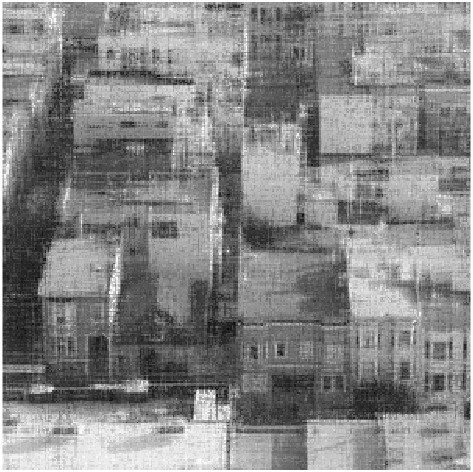
\includegraphics[width=\linewidth]{\mapa/rezTNNM1.png}
        \caption{Rekonstrukcija s parametrom 1.}
    \end{subfigure}
    \hfill
    \begin{subfigure}{0.325\linewidth}
        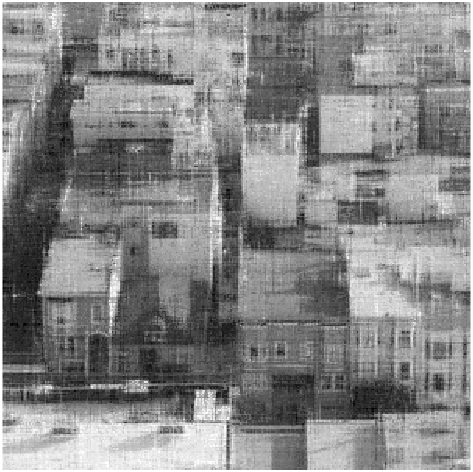
\includegraphics[width=\linewidth]{\mapa/rezTNNM5.png}
        \caption{Rekonstrukcija s parametrom 5.}
    \end{subfigure}
    \hfill
    \begin{subfigure}{0.325\linewidth}
        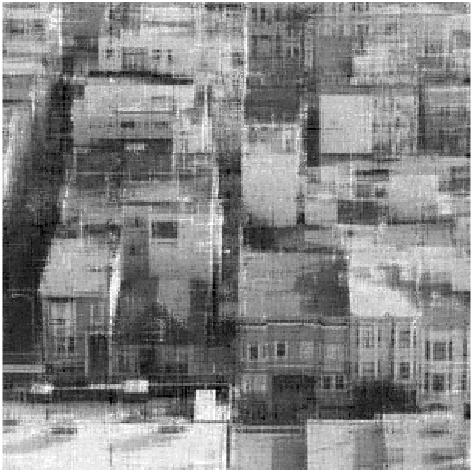
\includegraphics[width=\linewidth]{\mapa/rezTNNM12.png}
        \caption{Rekonstrukcija s parametrom 12.}
    \end{subfigure}
\end{figure}

\begin{figure}[h]
    \centering
    \begin{tabular}{|c|c|c|}
        \hline
        Parameter & Napaka & Čas izvajanja \\
        \hline
        1 & $5.70 \times 10^{3}$ & 35.9s \\
        5 & $5.46 \times 10^{3}$ & 481s \\
        12 & $5.27 \times 10^{3}$ & 930s \\
        \hline
    \end{tabular}
    \caption{Rezultati rekonstrukcije algoritma TNNM za različne parametre.}
\end{figure}
